\documentclass[uplatex,dvipdfmx,a4paper,twocolumn,base=11pt,jbase=11pt,ja=standard]{bxjsarticle}

% ===== IPSJ =====
\usepackage{ipsj}

% ===== 基本パッケージ(多くの論文で使用)=====
\usepackage[dvipdfmx]{graphicx}
\usepackage{tabularray}
\usepackage{float}
\usepackage{enumitem}
\usepackage{multirow}

% ===== 図表間隔(標準より少し詰める:崩れにくい安全値)=====
\setlength{\abovecaptionskip}{2pt}
\setlength{\belowcaptionskip}{2pt}
\setlength{\intextsep}{4pt}
\setlength{\textfloatsep}{6pt}

% ===== 段落間隔 =====
\setlength{\parskip}{3pt}

% ===== タイトル =====
\title{論文タイトルをここに記入}

% ===== 著者 =====
\author{%
著者A\textsuperscript{†}\hspace{0.6em}%
著者B\textsuperscript{†}\hspace{0.6em}%
著者C\textsuperscript{†}}

\date{}

\begin{document}

\makeatletter
\twocolumn[
  \begin{center}
    {\LARGE \@title \par}
    \vskip 0.5em
    {\normalsize \@author \par}
    \vskip 0.3em
    {\small \textsuperscript{‡} 所属機関名}
  \end{center}
  \vspace{1.5em}
]
\makeatother

% ===== 英語情報(任意)=====
%配列の番号に対応したダガーマークつける
%0 = ダガーなし, 1 = *, 2 = †, 3 = ‡, 4 以降も自動でマークつく
\renewcommand{\thefootnote}{\fnsymbol{footnote}}% 脚注を †, ‡, § ... にする
\footnotetext[0]{Paper Title in English}%英語タイトル
\footnotetext[2]{Author A, Author B, Author C}%英語著者
\footnotetext[3]{Affiliation in English}%英語所属

% =====================================================
\section{背景}
本文をここに記述する\cite{sample1}.
図\ref{fig:eng}, 表\ref{tab:test}に示す.
\begin{figure}[H]
\centering
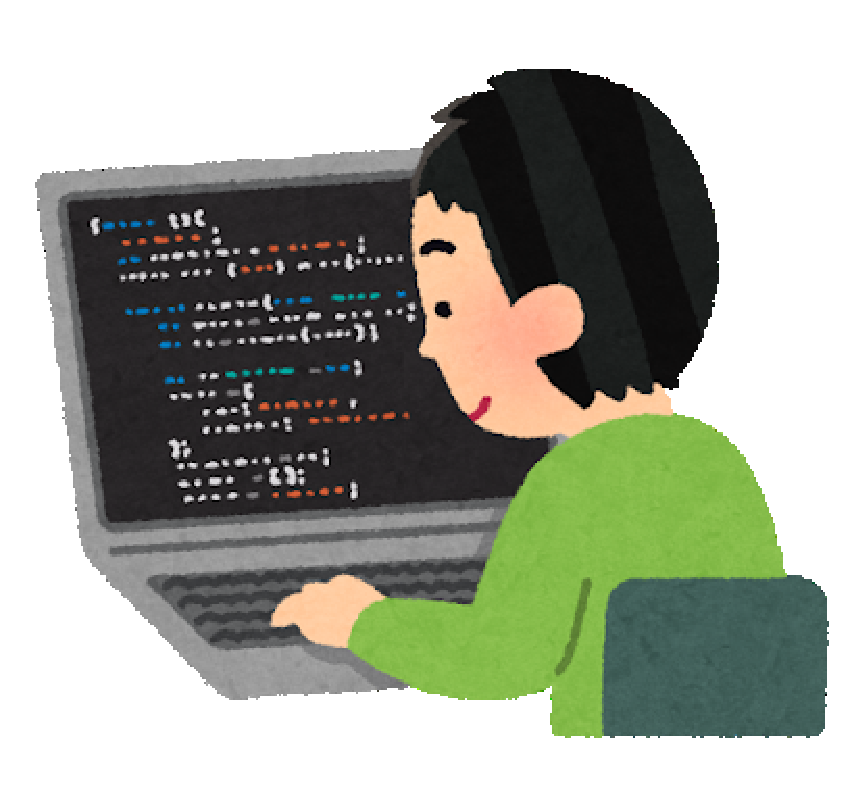
\includegraphics[width=70mm]{fig/man.eps}
\caption{エンジニア}
\label{fig:eng}
\end{figure}



\begin{table}[H]
  \centering
  \caption{実験結果}
  \label{tab:test}
  \begin{tabular}{ccc} \hline
   手法 & 数値 &  hoge\\ \hline
   A & 10.6 & huga \\
   B & 20.0 & hogehuga \\ \hline
\end{tabular}
\end{table}

\section{目的}
本文をここに記述する.

\section{提案手法}
本文をここに記述する.

\section{実験}
本文をここに記述する.

\section{結果}
本文をここに記述する.

\section{結論}
本文をここに記述する.

% =====================================================
{\small
\begin{thebibliography}{99}

\bibitem{sample1}
著者名, “論文タイトル”, 学会名, 年.

\bibitem{sample2}
Author, “Paper Title”, Conference/Journal, Year.

\end{thebibliography}
}

\end{document}